\documentclass{Phyport}

\usepackage{hyperref}
\hypersetup{
    colorlinks=true,
}
% 选用宏（如有额外需要的宏包请在此添加）
\usepackage{float}       % 提供 [H] 选项
\usepackage{booktabs}    % 三线表
\usepackage{amsmath}     % 数学公式
\usepackage{caption}     % 标题设置
\usepackage{siunitx}     % SI 单位排版
 %选用宏
\usepackage[european]{circuitikz}

\exname{交流电路功率因数实验} %实验名称
\extable{5} %实验桌号
\instructor{杨佳楠} %指导教师
\class{电科2502} %班级
\name{管云哲} %姓名
\stuid{3250104519} %学号

\nyear{2026} %年
\nmonth{11} %月
\nday{3} %日
\nweekday{二} %星期几

\redate{} %如有实验补做，补做日期
\resitu{} %情况说明：

\begin{document}
\setcounter{page}{1}
\makecover

\section{预习报告（10分）}
（注：将已经写好的“物理实验预习报告”内容拷贝过来）

\subsection{实验综述（5分）}
（自述实验现象、实验原理和实验方法，包括必要的光路图、电路图、公式等。不超过500字。）

实验现象：闭合开关，启辉器放电使灯丝预热；启辉器随后断开，镇流器产生高压脉冲点亮灯管，之后镇流器起限流作用。并联电容后，总电流随电容增大先减小后增大。

实验原理：交流电路的平均功率为 $P=UI\cos\varphi$，其中 $\cos\varphi=P/(UI)$ 称为功率因数。日光灯是电感性负载，可等效为灯管电阻 $R$ 与镇流器电感 $L$、内阻 $r$ 串联。灯管电流 $I_L$ 滞后总电压 $U$ 相位角 $\varphi$，故 $\cos\varphi<1$。在负载两端并联电容 $C$ 后，电容电流 $I_C$ 超前 $U$ 相位 $90^\circ$，总电流 $I=I_L+I_C$。若 $C$ 取值合适，总电流减小，相位差 $\varphi'<\varphi$，功率因数提高；$C$ 过大时总电流转为容性，$\cos\varphi$ 反而下降。

\begin{figure}[H]
    \centering
    \begin{minipage}[b]{0.62\linewidth}
        \centering
        \begin{circuitikz}[european, scale=0.72, transform shape]
            % 电源
            \draw (0,0) to[sV, l=$U$] (0,3.2);
            % 电压表
            \draw (0,3.2) -- (1.4,3.2) to[rmeter, t=$V$] (1.4,0) -- (0,0);
            % 功率表与电流表
            \draw (1.4,3.2) -- (2.4,3.2)
                  to[rmeter, t=$W$] (3.9,3.2)
                  to[rmeter, t=$A$] (5.4,3.2)
                  -- (6.4,3.2);
            % 并联电容支路
            \draw (6.4,3.2) to[vC, l=$C$] (6.4,0);
            % 镇流器
            \draw (6.4,3.2) -- (7.2,3.2) to[american inductor, l=$M$] (8.6,3.2) -- (9.4,3.2);
            % 灯管
            \draw (9.4,3.2) to[lamp, l_=$L$] (9.4,0.8) -- (9.4,0);
            % 启辉器
            \draw (9.4,3.2) -- (11,3.2)
                  to[lamp, l=$S$] (11,0.8)
                  -- (9.4,0.8);
            % 返回总线
            \draw (11,0.8) -- (11,0) -- (0,0);
            \node[circ] at (6.4,3.2) {};
            \node[circ] at (9.4,3.2) {};
            \node[circ] at (9.4,0.8) {};
        \end{circuitikz}\\[-1mm]
        {\small (a) 实验电路}
    \end{minipage}\hfill
    \begin{minipage}[b]{0.34\linewidth}
        \centering
        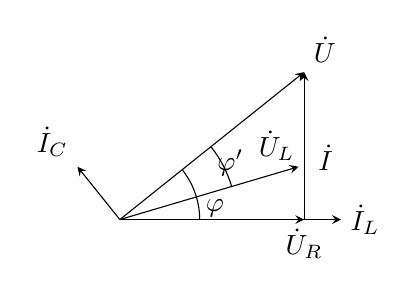
\begin{tikzpicture}[scale=0.78, >=stealth]
            \draw[->] (0,0) -- (3.6,0) node[right] {$\dot I_L$};
            \draw[->] (0,0) -- (3.0,2.4) node[above right] {$\dot U$};
            \draw[->] (0,0) -- (3.0,0) node[below] {$\dot U_R$};
            \draw[->] (3.0,0) -- (3.0,2.4) node[midway, left] {$\dot U_L$};
            \draw[->] (0,0) -- (-0.69,0.86) node[above left] {$\dot I_C$};
            \draw[->] (0,0) -- (2.91,0.86);
            \node at (3.35,1.0) {$\dot I$};
            \draw (1.3,0) arc (0:38.7:1.3);
            \node at (1.55,0.18) {$\varphi$};
            \draw (1.82,0.54) arc (16.5:38.7:1.9);
            \node at (1.80,0.92) {$\varphi'$};
        \end{tikzpicture}\\[-1mm]
        {\small (b) 相量图}
    \end{minipage}
    \caption{交流电路功率因数实验电路与并联电容前后的相量图}
    \label{fig:principle}
\end{figure}

实验方法：用电压表、电流表、功率表测额定电压下日光灯电路的 $U$、$I$、$P$，由 $\cos\varphi=P/(UI)$ 计算功率因数。将电容从 $1\,\mu\mathrm{F}$ 逐级增至 $7\,\mu\mathrm{F}$，计算各组的 $\cos\varphi$ 并作 $\cos\varphi$--$C$ 散点图，找出使 $\cos\varphi$ 最大的电容值。

\subsection{实验重点（3分）}
（简述本实验的学习重点，不超过100字。）

理解功率因数的物理意义及电感性负载 $\cos\varphi<1$ 的原因；掌握并联电容提高功率因数的方法；熟悉日光灯电路的结构与启辉、限流过程；学会用电压表、电流表、功率表测量并计算 $\cos\varphi$，由 $\cos\varphi$--$C$ 曲线确定最佳电容。

\subsection{实验难点（2分）}
（简述本实验的实现难点，不超过100字。）

日光灯启辉过程涉及启辉器与镇流器的配合，原理较抽象；电容需逐级接入，避免过大使总电流回升、功率因数下降。

\section{实验操作与原始数据（50分）}
（将有老师签名的“自备数据记录草稿纸”的扫描或手机拍摄图粘贴在下方，完整保留姓名，学号，教师签字和日期。按老师的要求拍摄实验过程图，附在此处）

实验在强电条件下进行，连线由教师预先接好，全程未私自改接。主要操作步骤如下：
\begin{enumerate}
    \item 不接入电容，闭合总电源与日光灯开关，观察启辉器放电、灯管点亮及镇流器限流的过程。
    \item 在额定电压下，用电压表、电流表、功率表测量日光灯电路的 $U$、$I$、$P$，由 $\cos\varphi=P/(UI)$ 计算未补偿时的功率因数。
    \item 断电后接入电容，按电容值由小到大逐级切换；每次待读数稳定后，记录 $U$、$I$、$P$，并计算对应的 $\cos\varphi$。
    \item 比较各组的 $\cos\varphi$，找出使 $\cos\varphi$ 最大的电容值；改变电源频率，在 45、50、55\,Hz 下重复测量。
\end{enumerate}

实验原始数据记录如图~\ref{fig:rawdata} 所示。

\begin{figure}[H]
    \centering
    \includegraphics[width=0.72\linewidth, height=0.82\textheight, keepaspectratio]{原始数据.jpg}
    \caption{原始数据记录}
    \label{fig:rawdata}
\end{figure}

\section{结果与分析（30分）}
\subsection{数据处理与结果（20分）}
（列出数据表格、选择适合的数据处理方法、写出测量或计算结果。）

\subsubsection{电容器实测值}

实验所用的标称 1\,$\mu$F 与 2\,$\mu$F 电容，其实际值由电容表测得，见表~\ref{tab:cap}。各档并联电容值均按实际值相加，而非标称值。

\begin{table}[H]
    \centering
    \caption{电容器标称值与实测值}
    \label{tab:cap}
    \begin{tabular}{cccc}
        \toprule
        标称值 & A & B & C \\
        \midrule
        $1\,\mu$F & 0.9310 & 0.9058 & 0.7572 \\
        $2\,\mu$F & 1.698 & 1.714 & 1.677 \\
        \bottomrule
    \end{tabular}

    \vspace{2pt}
    {\small 单位：$\mu$F。}
\end{table}

\subsubsection{测量数据与功率因数}

按 $\cos\varphi=P/(UI)$ 逐点计算功率因数，结果见表~\ref{tab:45}--表~\ref{tab:55}。其中 $I$ 已由 mA 换算为 A 后代入。45\,Hz 下 $C=2.645\,\mu$F 一组按原始记录取值（录入表曾误记为 2.695\,$\mu$F）。55\,Hz 下 $C=3.242\,\mu$F 的一组读数在原始记录中作废，重测值为 $3.517\,\mu$F，故表中不计入该点。

\begin{table}[H]
    \centering
    \caption{$f=45$\,Hz 时的测量数据与功率因数}
    \label{tab:45}
    \small
    \setlength{\tabcolsep}{5pt}
    \begin{tabular}{cccccc}
        \toprule
        $C$ / $\mu$F & $I$ / mA & $U$ / V & $P$ / W & $\cos\varphi$ \\
        \midrule
        0.000 & 371.4 & 219.4 & 29.7 & 0.3645 \\
        0.931 & 314.5 & 219.6 & 30.3 & 0.4387 \\
        1.714 & 272.1 & 219.8 & 30.6 & 0.5116 \\
        2.645 & 228.5 & 220.0 & 30.8 & 0.6127 \\
        3.412 & 196.4 & 220.3 & 31.1 & 0.7188 \\
        4.343 & 170.2 & 220.5 & 31.3 & 0.8340 \\
        5.089 & 161.4 & 220.6 & 31.7 & 0.8903 \\
        6.020 & 169.9 & 220.6 & 31.5 & 0.8404 \\
        6.925 & 194.6 & 220.1 & 31.4 & 0.7331 \\
        \bottomrule
    \end{tabular}
\end{table}

\begin{table}[H]
    \centering
    \caption{$f=50$\,Hz 时的测量数据与功率因数}
    \label{tab:50}
    \small
    \setlength{\tabcolsep}{5pt}
    \begin{tabular}{cccccc}
        \toprule
        $C$ / $\mu$F & $I$ / mA & $U$ / V & $P$ / W & $\cos\varphi$ \\
        \midrule
        0.000 & 297.7 & 219.0 & 24.8 & 0.3804 \\
        0.931 & 240.6 & 219.4 & 24.9 & 0.4717 \\
        1.714 & 196.7 & 219.4 & 24.9 & 0.5770 \\
        2.645 & 152.5 & 220.1 & 25.0 & 0.7448 \\
        3.412 & 130.1 & 219.7 & 25.2 & 0.8816 \\
        4.343 & 129.3 & 219.6 & 25.0 & 0.8805 \\
        5.089 & 151.6 & 219.3 & 25.2 & 0.7580 \\
        6.020 & 194.6 & 219.0 & 25.1 & 0.5890 \\
        6.925 & 247.1 & 219.2 & 25.2 & 0.4653 \\
        \bottomrule
    \end{tabular}
\end{table}

\begin{table}[H]
    \centering
    \caption{$f=55$\,Hz 时的测量数据与功率因数}
    \label{tab:55}
    \small
    \setlength{\tabcolsep}{5pt}
    \begin{tabular}{cccccc}
        \toprule
        $C$ / $\mu$F & $I$ / mA & $U$ / V & $P$ / W & $\cos\varphi$ \\
        \midrule
        0.000 & 250.9 & 218.4 & 19.6 & 0.3577 \\
        0.803 & 189.1 & 218.7 & 20.1 & 0.4860 \\
        1.773 & 134.3 & 218.5 & 20.2 & 0.6884 \\
        3.517 & 106.9 & 217.5 & 20.3 & 0.8731 \\
        4.320 & 146.6 & 217.7 & 20.5 & 0.6423 \\
        5.153 & 193.8 & 217.6 & 20.3 & 0.4814 \\
        5.956 & 253.6 & 217.6 & 20.5 & 0.3715 \\
        \bottomrule
    \end{tabular}
\end{table}

未并联电容时，45、50、55\,Hz 下的功率因数分别为 0.3645、0.3804、0.3577，对应的相位角约为 $68.6^\circ$、$67.6^\circ$、$69.0^\circ$，说明日光灯确为感性负载。接入电容后，总电流先减小后增大，功率因数先升高后降低，见图~\ref{fig:cosphi} 与图~\ref{fig:current}。这是因为电容电流与感性无功电流反相，先抵消部分无功分量；电容过大后无功电流反向，总电流重新增大，功率因数下降。

\begin{figure}[H]
    \centering
    \includegraphics[width=0.72\linewidth]{cosphi_vs_C.pdf}
    \caption{不同频率下 $\cos\varphi$ 随电容 $C$ 的变化}
    \label{fig:cosphi}
\end{figure}

\begin{figure}[H]
    \centering
    \includegraphics[width=0.72\linewidth]{current_vs_C.pdf}
    \caption{不同频率下总电流 $I$ 随电容 $C$ 的变化}
    \label{fig:current}
\end{figure}

\subsubsection{最佳电容与理论值的比较}

日光灯等效为电阻 $R$ 与电感 $L$ 串联，未补偿时的无功功率为
\begin{equation}
    Q_L=P_0\tan\varphi_0,
    \label{eq:QL}
\end{equation}
其中 $P_0$、$\varphi_0$ 为未接电容时的功率与相位角。并联电容的无功功率为
\begin{equation}
    Q_C=\frac{U^2}{X_C}=\omega C U^2=2\pi fCU^2.
    \label{eq:QC}
\end{equation}
令 $Q_C=Q_L$，得使功率因数最高的理论电容
\begin{equation}
    C_{\text{理}}=\frac{P_0\tan\varphi_0}{2\pi fU_0^2}.
    \label{eq:Ctheory}
\end{equation}

表~\ref{tab:opt} 同时给出实测最大点、三点抛物线插值所得顶点与理论值。由于电容按固定档位切换，相邻档间隔约 0.6\,$\mu$F，直接取最大点只能把最佳值限定在一个档位内；对最优点及左右相邻点作抛物线插值，可减小档位离散带来的偏差。

\begin{table}[H]
    \centering
    \caption{最佳电容的实测值与理论值}
    \label{tab:opt}
    \small
    \setlength{\tabcolsep}{4pt}
    \begin{tabular}{cccccc}
        \toprule
        $f$ / Hz & $C_{\max}$ / $\mu$F & $\cos\varphi_{\max}$ & $C_{\text{插值}}$ / $\mu$F & $C_{\text{理}}$ / $\mu$F & 相对偏差 / \% \\
        \midrule
        45 & 5.089 & 0.8903 & 5.21 & 5.58 & $-6.6$ \\
        50 & 3.412 & 0.8816 & 3.87 & 4.00 & $-3.3$ \\
        55 & 3.517 & 0.8731 & 2.99 & 3.10 & $-3.8$ \\
        \bottomrule
    \end{tabular}
\end{table}

由表~\ref{tab:opt} 可见，插值所得最佳电容与理论值相差 3.3\%--6.6\%，且随频率升高而减小：$f$ 增大时 $X_C=1/(2\pi fC)$ 减小，只需较小的电容即可提供相同的无功电流，故 $C_{\text{理}}\propto 1/f$。实测最佳点也呈同一趋势，说明并联电容补偿的规律与理论一致。

需要指出，补偿后的最大功率因数仅为 0.87--0.89，并未接近 1。其原因主要有两点：一是日光灯电流为非正弦波，含较多谐波，$P/(UI)$ 给出的是包含谐波畸变的功率因数，即使基波无功完全补偿，该值仍小于 1；二是镇流器存在铁损与铜损，并非纯电感，其等效串联电阻使相位角不能完全补偿。

\subsection{误差分析（10分）}
（运用测量误差、相对误差或不确定度等分析实验结果，写出完整的结果表达式，并分析误差原因。）

\subsubsection{功率因数的不确定度}

由 $\cos\varphi=P/(UI)$，按不确定度传递公式，相对不确定度为
\begin{equation}
    \frac{u(\cos\varphi)}{\cos\varphi}
    =\sqrt{\left(\frac{u_P}{P}\right)^2
    +\left(\frac{u_U}{U}\right)^2
    +\left(\frac{u_I}{I}\right)^2}.
    \label{eq:ucos}
\end{equation}
实验为单次读数，无重复测量，故只估计 B 类不确定度。取数字表的读数分辨力 $U$：0.1\,V、$I$：0.1\,mA、$P$：0.1\,W，按均匀分布 $u=\Delta/\sqrt{3}$，得 $u_U=0.058$\,V、$u_I=0.058$\,mA、$u_P=0.058$\,W。以各频率下功率因数最大点代入式~\eqref{eq:ucos}，结果见表~\ref{tab:u}。

\begin{table}[H]
    \centering
    \caption{最佳点功率因数的 B 类不确定度}
    \label{tab:u}
    \begin{tabular}{cccccc}
        \toprule
        $f$ / Hz & $P$ / W & $U$ / V & $I$ / mA & $\cos\varphi$ & $u(\cos\varphi)$ \\
        \midrule
        45 & 31.7 & 220.6 & 161.4 & $0.8903\pm0.0017$ & 0.0017 \\
        50 & 25.2 & 219.7 & 130.1 & $0.8816\pm0.0021$ & 0.0021 \\
        55 & 20.3 & 217.5 & 106.9 & $0.8731\pm0.0025$ & 0.0025 \\
        \bottomrule
    \end{tabular}
\end{table}

即
\begin{equation}
    \cos\varphi=
    \begin{cases}
        0.890\pm0.002, & f=45\,\mathrm{Hz},\\
        0.882\pm0.002, & f=50\,\mathrm{Hz},\\
        0.873\pm0.003, & f=55\,\mathrm{Hz}.
    \end{cases}
\end{equation}

最佳电容由档位离散决定，电容步进约 0.6\,$\mu$F，故 $C_{\text{插值}}$ 的分辨力约为 $\pm0.3\,\mu$F。取
\begin{equation}
    C_{\text{opt}}=
    \begin{cases}
        (5.2\pm0.3)\,\mu\mathrm{F}, & f=45\,\mathrm{Hz},\\
        (3.9\pm0.3)\,\mu\mathrm{F}, & f=50\,\mathrm{Hz},\\
        (3.0\pm0.3)\,\mu\mathrm{F}, & f=55\,\mathrm{Hz}.
    \end{cases}
\end{equation}

\subsubsection{误差来源分析}

\begin{enumerate}
    \item \textbf{日光灯的非线性}：灯管电阻随电流、温度变化，接入电容后灯管电压由 219\,V 升至 220.6\,V，$P$ 也由 29.7\,W 增至 31.7\,W。理论公式用未补偿时的 $P_0$、$\varphi_0$ 预测最佳电容，忽略了工作点的移动，这是实测值系统性偏小的主要原因之一。
    \item \textbf{电流的非正弦性}：日光灯电流含谐波，$P/(UI)$ 不等于基波相移因数。谐波使实测 $\cos\varphi$ 偏低，也解释了为什么补偿后最大功率因数只有 0.87--0.89。
    \item \textbf{镇流器的损耗}：镇流器线圈有铜阻和铁损，等效电路不是纯电感，其串联电阻消耗有功功率并使相位角偏移，$Q_L=P\tan\varphi_0$ 只是近似。
    \item \textbf{电容值的偏差与档位离散}：标称 1\,$\mu$F 的 C 组实测仅 0.7572\,$\mu$F，偏差达 $-24.3\%$；若按标称值计算，最佳电容将明显偏离。本实验已用实测值，但档位间隔仍限制了最佳点的分辨力。
    \item \textbf{仪表误差}：电压、电流、功率表均有准确度等级与零点漂移，功率表还受功率因数影响；实验未记录仪表等级，无法定量修正。读数末位估读也会引入随机误差。
    \item \textbf{电源与环境波动}：测量过程中电网电压在 217.5--220.6\,V 间变化，频率也可能有微小漂移；温度变化影响灯管与镇流器参数，使各点工作状态不完全一致。
\end{enumerate}

\section{实验探讨与思考题（10分）}
（对实验内容、现象和过程的小结，不超过100字。并解答教材或讲义或老师布置的思考题，请先写题干，再作答。）

本实验验证了并联电容补偿感性负载的规律：总电流先减小后增大，功率因数先升后降；最佳电容随频率升高而减小，实测与理论值相差 3.3\%--6.6\%。

\subsubsection{思考题 1}
\textbf{题干：}提高功率因数的意义何在？为什么并联电容能提高功率因数？并联的电容是否越大越好？

\textbf{解答：}提高功率因数的意义主要有四点。第一，提高用电利用率：电源设备的容量按视在功率 $S=UI$ 设计，功率因数越高，同一容量可输出的有功功率越大。第二，减少线路损耗：负载有功功率 $P$ 一定时，$I=P/(U\cos\varphi)$，$\cos\varphi$ 提高使线路电流减小，线路损耗 $I^2R$ 按电流平方下降。第三，改善电压质量：电流减小使线路阻抗上的电压降减小，末端电压更稳定。第四，降低用电成本：供电部门对低功率因数用户加收费用。

并联电容能提高功率因数，是因为电容电流 $\dot I_C$ 超前电压 $90^\circ$，而感性负载电流的无功分量滞后电压 $90^\circ$，两者相位相反。并联后总电流为
\begin{equation}
    \dot I=\dot I_R+\mathrm{j}(\dot I_L-\dot I_C),
\end{equation}
其无功分量被部分抵消，总电流减小，电流与电压的相位差 $\varphi'$ 减小，故 $\cos\varphi'$ 提高。并联电容不改变负载两端电压，也不改变负载本身的有功功率，只提供无功功率，因此是补偿感性负载的合适方法。

并联电容并非越大越好。当 $I_C=I_L$ 时无功分量完全抵消，功率因数达到最大；若继续增大电容，$I_C>I_L$，总电流转为容性，相位差反向增大，$\cos\varphi$ 反而下降，总电流重新增大。过补偿还会使线路电压升高，增加电容和开关设备的负担。因此应按负载的无功功率选择电容，使补偿后的功率因数接近 1 而不发生过补偿。

\subsubsection{思考题 2}
\textbf{题干：}在实验中，随着电容增加，电路的总电流的变化规律为由大变小再变大，试分析原因。

\textbf{解答：}把日光灯支路分解为有功分量 $I_R$ 和无功分量 $I_L$。有功分量由灯管和镇流器的电阻决定，在电压基本不变时近似恒定；无功分量由镇流器电感决定，滞后电压 $90^\circ$。并联电容后，电容电流 $I_C=\omega CU$ 超前电压 $90^\circ$，且随电容增大而线性增大。总电流的有效值为
\begin{equation}
    I=\sqrt{I_R^2+(I_L-I_C)^2}.
    \label{eq:Itotal}
\end{equation}
电容较小时，$I_C<I_L$，$(I_L-I_C)$ 随 $C$ 增大而减小，故 $I$ 减小；当 $I_C=I_L$ 时，$(I_L-I_C)=0$，$I$ 达到最小值 $I_R$，此时功率因数最高；电容继续增大，$I_C>I_L$，$(I_L-I_C)$ 的绝对值重新增大，总电流转为容性并再次增大。式~\eqref{eq:Itotal} 的抛物线形关系与图~\ref{fig:current} 的实验曲线一致。实际曲线的最小值不为零，是因为 $I_R$ 始终存在，且电流含谐波、灯管参数随电压变化。

\subsubsection{思考题 3}
\textbf{题干：}在进行功率因数补偿时，本实验采用并联电容器的方法，为什么不采用串联电容器的方法？

\textbf{解答：}串联电容会改变负载的工作条件。日光灯要求灯管与镇流器在额定电压下工作；若把电容与整个负载串联，电容上会产生电压降，负载两端电压低于电源电压，灯管可能无法启辉或亮度不足，镇流器的限流条件也被破坏。串联电容还会使总阻抗、总电流和相位关系随负载变化，不能单独调节无功功率，补偿量难以控制。

并联电容则不同：电容支路与负载并联，负载两端电压仍为电源电压，负载的有功功率和工作状态基本不变；电容只向电路提供超前无功电流，抵消感性无功电流。并联补偿还可以分级投切，按负载变化增减电容，运行灵活，且某一电容支路故障不影响负载供电。因此功率因数补偿普遍采用并联电容器，而不采用串联电容器。

{\fangsong 注意事项：
\begin{enumerate}[label=\arabic*.]
    \item 用PDF格式上传“实验报告”，文件名：学生姓名+学号+实验名称+周次。
    \item “实验报告”必须递交在“学在浙大”本课程内对应实验项目的“作业”模块内。
    \item “实验报告”成绩必须在“浙江大学物理实验教学中心网站”-“选课系统”内查询。
    \item 教学评价必须在“浙江大学物理实验教学中心网站”-“选课系统”内进行，学生必须进行教学评价，才能看到实验报告成绩，教学评价须在本次实验结束后3天内进行。
\end{enumerate}}
\begin{center}
    \fbfangsong{浙江大学物理实验教学中心制}
\end{center}
\end{document}
